Essa seção apresenta a estrutura geral do VANT como aeronave escolhida, seus materiais e seu protótipo.
\subsubsection{Escolha da aeronave}

Para escolha da aeronave, que atende à todas as necessidades impostas pelo projeto, deve-se considerar quais características a aeronave possui.
A escolha levou em consideração a melhor aeronavegável e que pudesse suportar a maior carga possível.

O VANT precisa atender o transporte de equipamento hospitalar, as possíveis aeronaves para essa função são: VANT asa fixa e VANT asa 
rotativa (multirotores).

Os VANT’s de asa fixa, no caso, os aviões não tripulados, apesar de serem rápidos e possuírem um longo alcance de voo, para transporte de carga,
exige um tamanho grande de asa, A envergadura do VANT muda com relação ao peso, e como a carga de transporte é considerada elevada, o 
comprimento da asa teria que ser muito grande, como o próprio avião. A aterrisagem é outro fator que dificulta, pois os aeromodelos 
exige um espaço aberto com uma pista de pouso para conseguirem descer. As dimensões da pista é uma grande dificuldade, pois a pista
precisa ser maior que o modelismo e não é em qualquer lugar que ele pode realizar esse procedimento, devido o grande risco,
tornando-se perigoso. Não é aconselhado pousos próximo de pessoas e em curtos espaços.

Os multirotores vêm aumentando no mercado nos últimos anos. Os multirotores são estruturas com vários motores (dois ou mais rotores) e 
esses motores são fixos em uma estrutura, e os motores não precisão de ajustes como nos helicópteros. O \textit{Roll} e o \textit{Pitch} é feito 
apenas com a rotação do motor. Além disso, não há rotor de cauda, utilizada para fornecer controle de guinada e contrariar o torque posto 
para fora por dirigir o principal rotor em um helicóptero. Por serem simétricos, o controle de um multirotor é mais fácil e mais estável. O
que permite uma decolagem e uma aterrissagem mais prática e com menos espaço.

Os multirotores voam através da utilização de dois princípios básicos: elevação (\textit{lift}) e torque. Multirotores são verdadeiramente
um grande exercício de física newtoniana: toda ação tem uma reação de mesma intensidade e sentido oposto. O multirotor usa  hélices 
diferentes e a contra-rotação para  manter o corpo  estável, pois dessa forma mantem-se a conservação do momento angular \cite{audronis}. 
Nos helicópteros tem-se o rotor de calda para evitar que o corpo girar e perca a estabilidade, o rotor de cauda é implementado de forma que 
mantenha a conservação de momento no helicóptero. 

Na figura \ref{fig:rotacao} é possível ver um multirotor, a representação mostra como que as hélices devem girar para que seja possível 
um voo estável. Esse princípio é aplicado a todos os multirodores e não apenas no quadrirotor. Sempre as hélices opostas (as que ficam 
uma em frente da outra) devem girar em mesma direção caso deseja-se entrar para frente.


\begin{figure}[H]
    \centering
      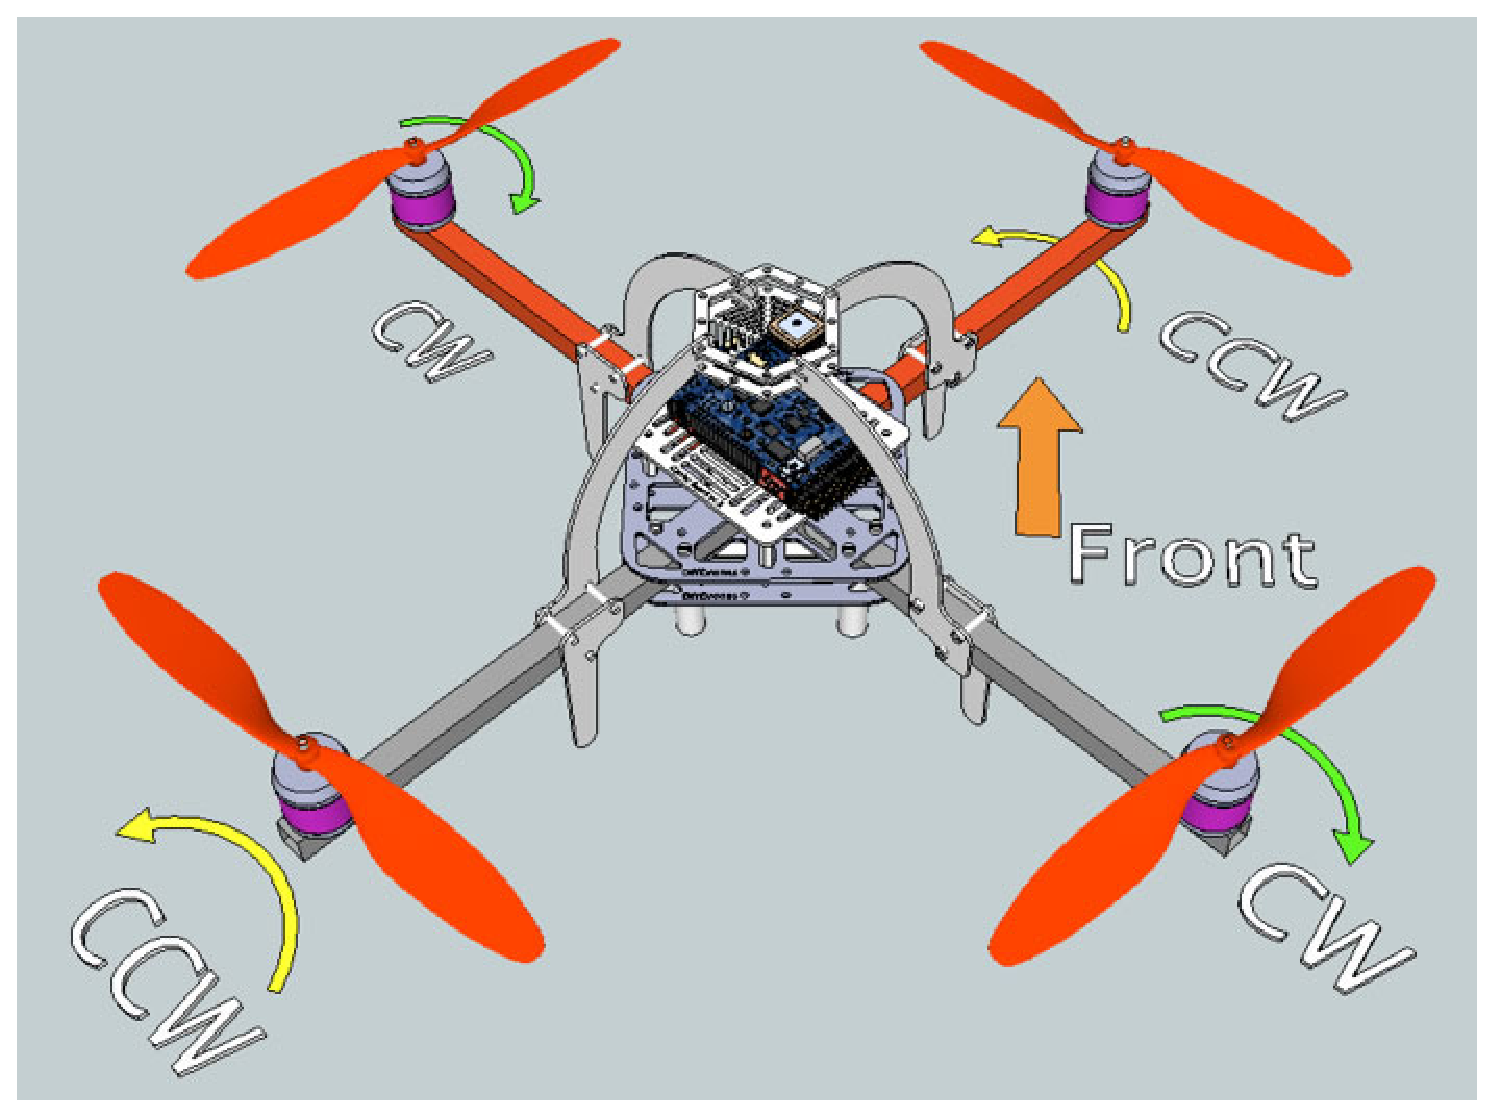
\includegraphics[keepaspectratio=true,scale=0.5]{figuras/rotacao.eps}
    \caption[Diagrama  de rotação das hélices de um quadricoptero estável]{Diagrama  de rotação das hélices de um quadricoptero estável. Fonte \cite{audronis}}
    \label{fig:rotacao}
\end{figure}

O multirotor possui a mobilidade de ir para frente, para trás e de lado para o outro mudando apenas o sentido temporariamente das hélices
como representado na imagem \ref{fig:gira}. Ao realizar essas manobrar ele pode inclinar o multirotor, alterando a direção do empuxo fornecido 
pelos rotores dessa forma realizando a curva mostrado na imagem \ref{fig:guinada}.

\begin{figure}[H]
    \centering
      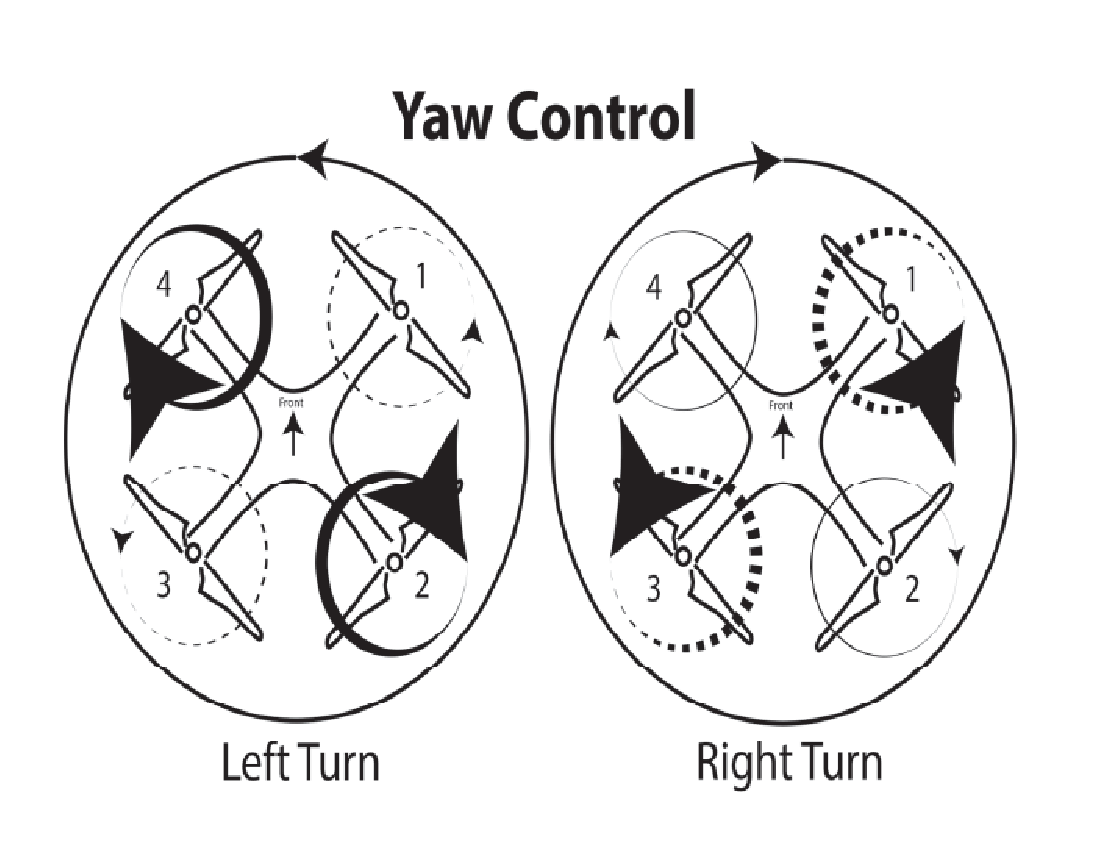
\includegraphics[keepaspectratio=true,scale=0.5]{figuras/gira.eps}
    \caption{Diagrama de gira para esquerda e para direita. Fonte \cite{audronis}}
    \label{fig:gira}
\end{figure}

\begin{figure}[H]
    \centering
      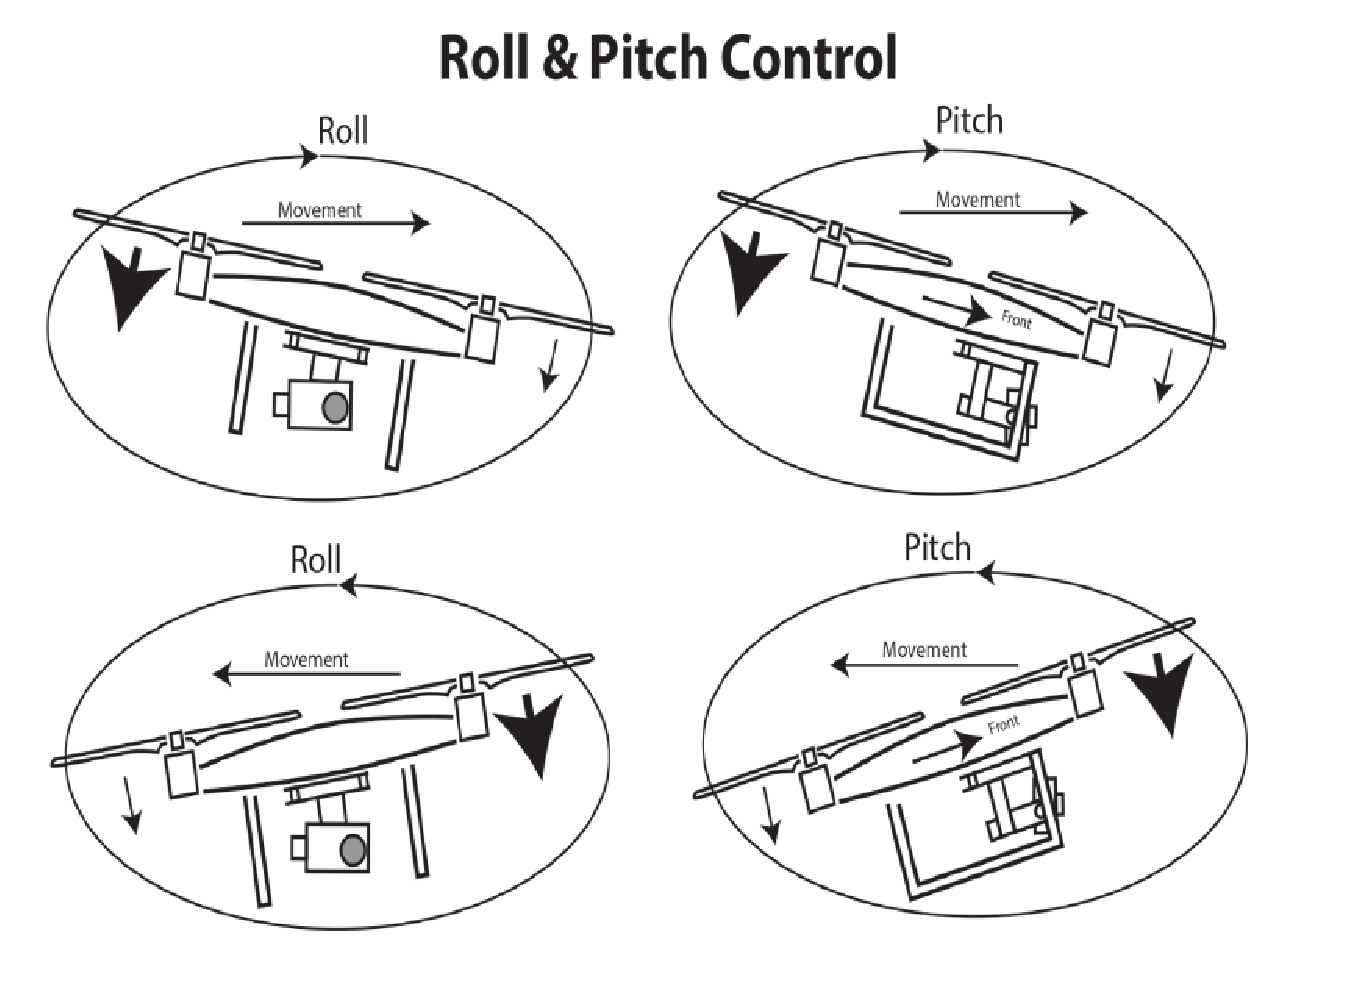
\includegraphics[keepaspectratio=true,scale=0.5]{figuras/guinada.eps}
    \caption[Diagrama de guinada e rolagem de um quadricóptero.]{Diagrama de guinada e rolagem de um quadricóptero. Fonte \cite{audronis}}
    \label{fig:guinada}
\end{figure}
A desvantagem de utilizar  os multirotores  é a  falta  de aerodinâmica,  dessa for o tempo de voo é reduzido significativamente e a baixa  
eficiência dos motores.  Contudo, para transporte de equipamento hospitalar, mas para o projeto será ideal, pois sua estabilidade, 
facilidade de controle, o tamanho reduzido e grande mobilidade compensa a falta de eficiência. A aplicação não precisa de percorrer 
distâncias muito grande, com isso ele se encaixa perfeitamente nas especificações.
\subsubsection{Especificação do VANT escolhido}

O multirotor escolhido para esse projeto é o de oito hélices, ou octocóptero. Em- bora oito rotores ofereçam mais estabilidade, também diminuem 
o tempo de voo, porque aumenta a quantidade de corrente exigida para alimentar todos os motores.  O projeto exige uma maior capacidade de carga, pois os equipamentos utilizados são considerados de alta densidade. Para que as especificações fossem atendidas, decidiu-se utilizar essa especificação por sua estabilidade e maior capacidade de gerar empuxo.

O motor escolhido é o motor Tarot 4114 \textit{High Power Brushless} (sem escova), que é um motor de altas rotações, representado na figura 
\ref{fig:tarot2}.

\begin{figure}[H]
    \centering
      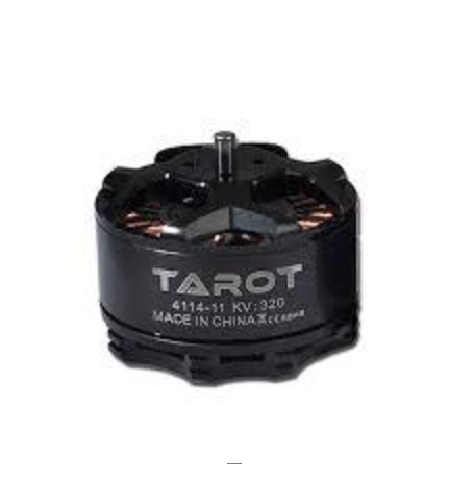
\includegraphics[keepaspectratio=true,scale=0.5]{figuras/tarot2.eps}
    \caption{Motor Tarot 4114 \textit{High Power Brushless}. \cite{tarot}}
    \label{fig:tarot2}
\end{figure}
\vfill
Este motor é comumente utilizado em  multirotores, um exemplo o modelo US 1000 de filmagens. Ele possui capacidade de gerar um empuxo de até
2.5 kg e uma outra característica desse tipo de motor é a magnetização do rotor ser por imãs permanentes. Motores de corrente contínua 
possuem vários benefícios em relação aos motores com escova, dentre algumas estão: melhor característica velocidade x torque, maiores
eficiência, vida útil, taxa de velocidade e é mais silencioso \cite{nascimento}.

\begin{figure}[H]
    \centering
      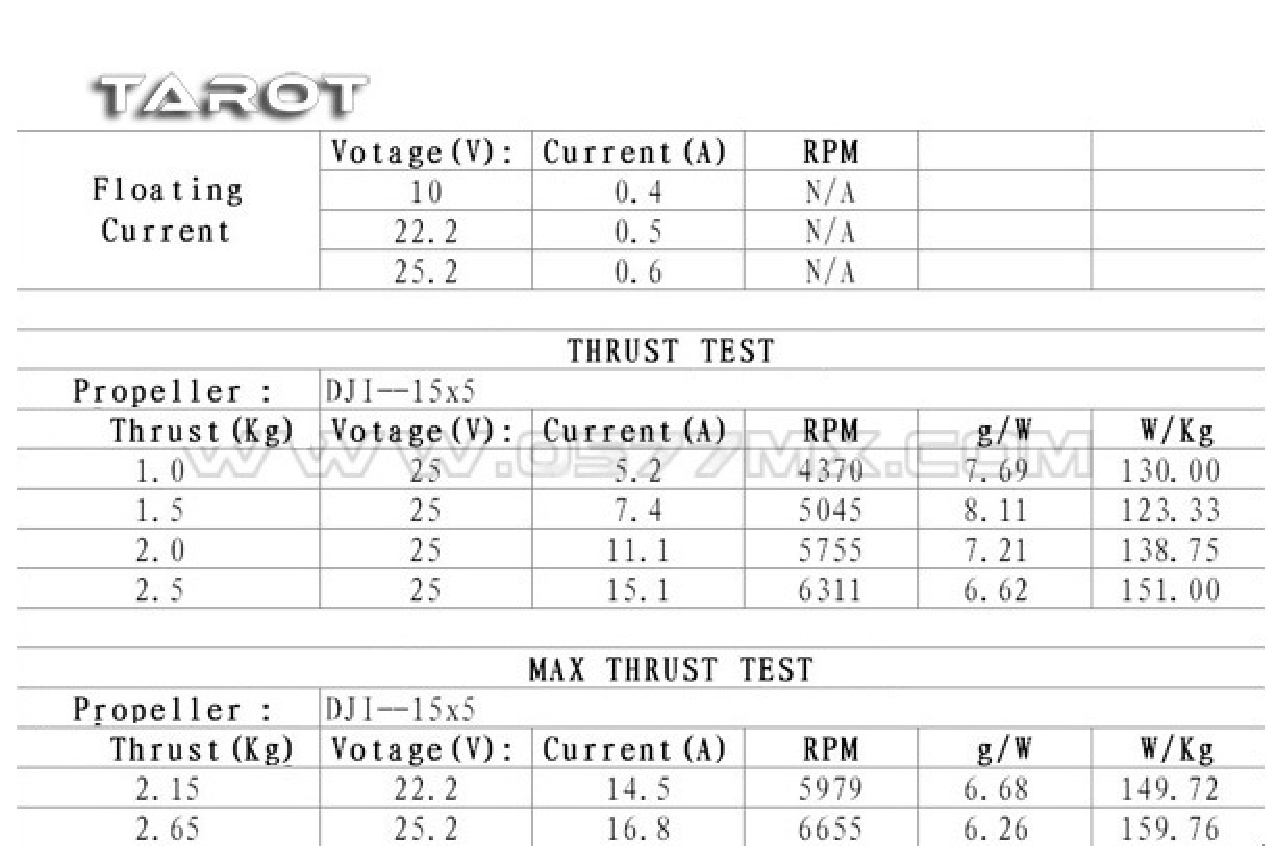
\includegraphics[keepaspectratio=true,scale=0.5]{figuras/tarot.eps}
    \caption{Quadro de relação de um motor 4114.\cite{tarot}}
    \label{fig:tarot}
\end{figure}

A hélice é um conjunto de pás com o mesmo centro, que ao serem rotacionadas criam um deslocamento do ar em direção ao solo e pelo efeito da 
terceira lei de Newton o conjunto é impulsionado para o sentido oposto, dessa forma cria-se a sustentação necessária para o vôo.  
Quanto maior o passo da hélice, maior a velocidade alcançada  pela aeronave e mais lenta é a resposta à manobras \cite{VIOLATO}. 
Para nossa proposta, utilizou-se uma hélice de tamanho médio, pois a aplicação necessita de velocidade e também de uma mobilidade boa.
A hélice escolhida é a 15x5 5.E \textit{Carbon  Fiber  Propellers  L/H  and  R/H  Rotation  Suits DJI}.

\begin{figure}[H]
    \centering
      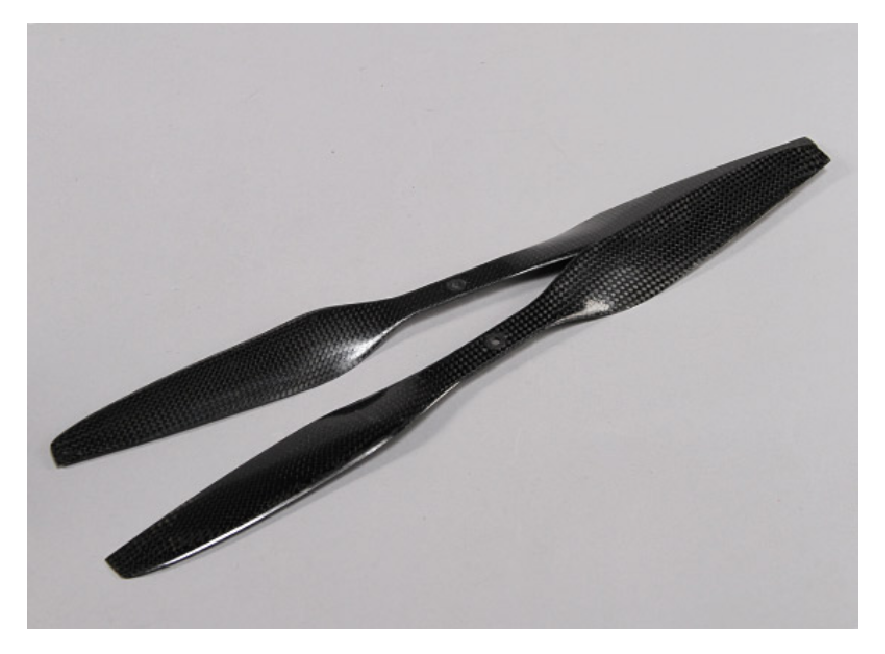
\includegraphics[keepaspectratio=true,scale=0.5]{figuras/diagramaEstru.eps}
    \caption[\textit{Carbon Fiber Propellers L/H and R/H Rotation Suits DJI.}]{\textit{Carbon Fiber Propellers L/H and R/H Rotation Suits DJI.} \cite{pinto}}
    \label{fig:elice}
\end{figure}

O ESC (\textit{Eletronic speed control}) é quem torna possível o voo, é o controle eletrônico da velocidade, ele é o responsável por 
alimentar o motor e mandar a potência que é necessária, ele impede sobrecarga nos motores, funcionando também como um módulo de proteção. 
Os ESCS são específicos para cada motor, eles devem ser dimensionados corretamente, pois um dimensionamento indevido pode ocasionar em uma 
sobrecarga nos motores e queimá-los.  Cada motor tem o seu ESC individual, dessa forma é possível controlar individualmente cada motor. Os 
ESCs são ligados no circuito do VANT como mostra a figura \ref{fig:diagramaEstru}.
 

\begin{figure}[H]
    \centering
      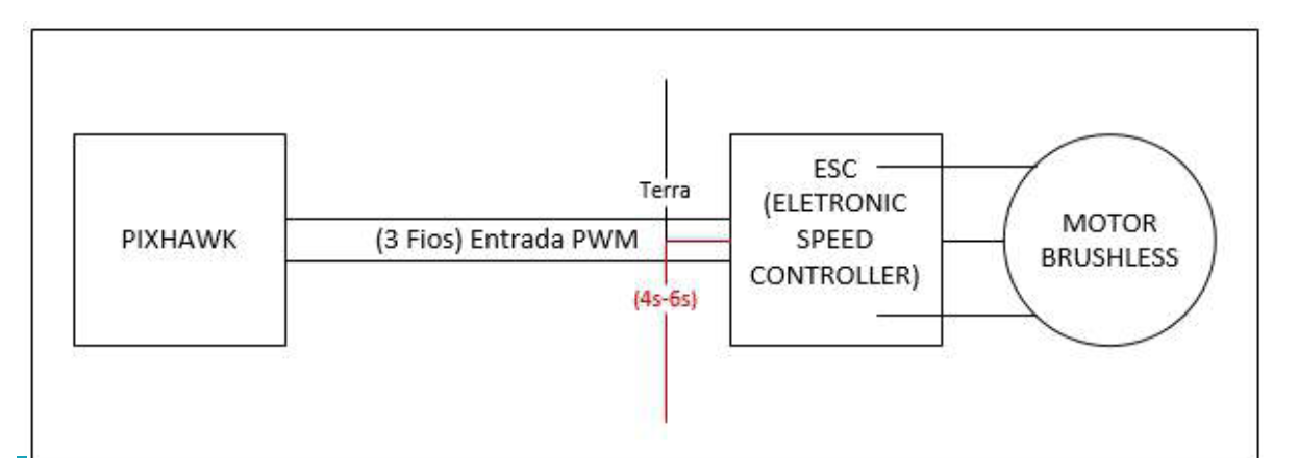
\includegraphics[keepaspectratio=true,scale=0.5]{figuras/elice.eps}
     \caption{Esquemático  de conexão e funcionamento  do ESC\cite{dji}}
    \label{fig:diagramaEstru}
\end{figure}

\subsubsection{Escolha dos materiais}

A escolha de determinados materiais nos projeto da engenharia é determinante para um bom projeto, para a escolha leva-se em  consideração 
os ambientes em que serão operados, dessa forma é possível entender o comportamento dos materiais diante a aplicação, dessa forma podendo 
garantir uma maior solidez e confiabilidade no projeto.

Os componentes que farão parte do drone serão os motores de alto desempenho, as hélices, componentes elétricos e a estrutura do corpo. 
Esta delimitação de materiais que satisfazem as necessidades do drone foi feita levando  em conta o tipo dos esforços que estarão  presentes,  
por exemplo, na decolagem, aterrissagem  e durante o tempo  de voo. Para as hélices e para  o motor foi escolhida  a fibra de carbono  e
para  o restante dos materiais da estrutura a opção foi da fibra de vidro.

A justificativa para a escolha destes materiais foi baseada de acordo com o módulo de elasticidade, a ductilidade, o limite de
resistência à tração e a tenacidade. 

Para que seja possível a visualização da comparação feita, as características citadas acima serão brevemente explicadas.


\begin{figure}[H]
    \centering
      \includegraphics[keepaspectratio=true,scale=0.7]{figuras/grafico-tensao.eps}
    \caption{Gráfico Tensão-Deformação.Fonte: \cite{callister}}
    \label{fig:grafico-tensao}
\end{figure}

O módulo de elasticidade é a inclinação da região de comportamento elástico inicial da curva, ou seja, o coeficiente linear da reta antes de atingir a região de deslizamento de discordâncias.
\begin{equation}
E =\frac{\Delta y}{\Delta x}
\end{equation}
A ductilidade é a medida do grau de deformação plástico que foi suportada até a fratura(F). Pode ser expressa quantitativamente como a porcentagem do alongamento percentual.
\begin{equation}
AL\% =\frac{lf - lo}{lo} * 100
\end{equation}
\begin{center}
lf = comprimento final e lo = comprimento inicial
\end{center}

O limite de resistência à tração está caracterizado no gráfico como início da ruptura e indica o valor máximo de tensão que pode ser suportado por uma estrutura sob tração.
A tenacidade é definida como sendo a habilidade de um material absorver energia e se deformar plasticamente antes de fraturar.

\begin{figure}[h]
    \centering
      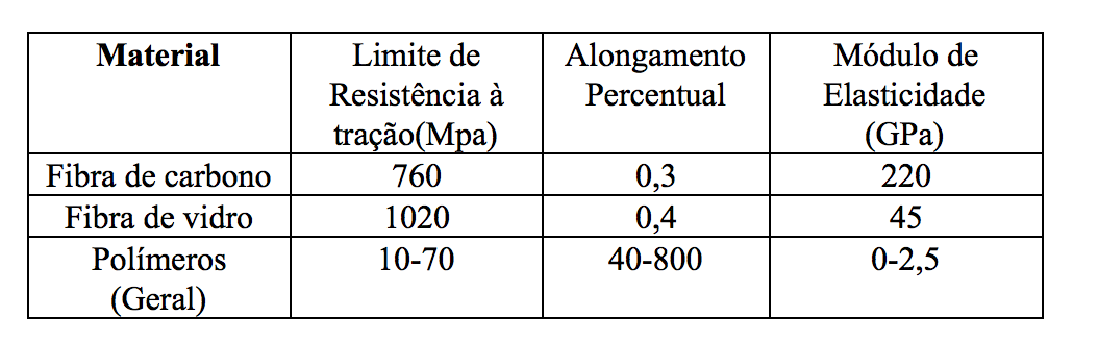
\includegraphics[keepaspectratio=true,scale=0.7]{figuras/graficoRelacao.eps}
    \caption{ Relação de materiais}
    \label{fig:graficoRelacao}
\end{figure}

Os materiais escolhidos, fibra de vidro e carbono, são determinados como materiais compósitos. As características destes incluem em pegar as melhores carcteristicas de variados materiais e junta-las para que se tenha um melhor desempenho no geral. 

Portanto, a escolha dos materiais do drone pode ser explicada de acordo com a tabela acima e com as explicações teóricas do que cada característica representa. 

Embora o alongamento percentual dos materiais poliméricos em geral seja muito maior do que os dos materiais ecolhidos para a aplicação do drone, esta característica é exibida no domínio plástico, ou seja, o material não se romperá mais perderá a qualidade devido a uma quantidade significativa de deformação.

Como conclusão do material a ser utilizado, é interessante partes da estrutura, como os braços, frame central, hélices e trem de pouso, utilizando fibra de carbono. Partes como a carcaça e componentes eletrônicos, poderão ser utilizados polímeros em geral. 

\subsubsection{Construção do VANT}

Considerando a parte mais importante do projeto, o desfibrilador será acoplado no VANT, na qual suas medidas são utilizadas como referência para modelagem do frame central.  A modelagem dos braços e hélices do drone,  não serão necessários, devido ao fato que eles serão utilizados do modelo similar ao de um VANT S1000

Para inicio da construção do VANT, consideramos as medidas de um DEA (Desfibrilador externo automático) vendido no mercado, chamado \textit{HeartSine samaritan PAD SAM 300P}  como o representado na figura \ref{fig:heart}:

\begin{figure}[H]
    \centering
      \includegraphics[keepaspectratio=true,scale=0.2]{figuras/heart.eps}
    \caption{ HeartSine samaritan PAD SAM 300P. Fonte: \cite{aedsingapore}}
    \label{fig:heart}
\end{figure}

O frame central projetado será baseado no frame central do S1000, porém adaptado ao desfibrilador e ao reanimador ventilatório, como é possível ver na figura 19: 

\begin{figure}[H]
    \centering
      \includegraphics[keepaspectratio=true,scale=0.5]{figuras/framecentral.eps}
    \caption{ Frame central S1000. Fonte: \cite{heliguy}}
    \label{fig:framecentral}
\end{figure}


Como as medidas, seguindo o manual, do frame central do S1000 é 337.5mm da ponta de um braço até outra, para o nosso projeto, será aumentado  200mm em relação ao centro, 100mm para um lado e 100mm par outro. Como mostra na figura \ref{fig:drawing}:

\begin{figure}[H]
    \centering
      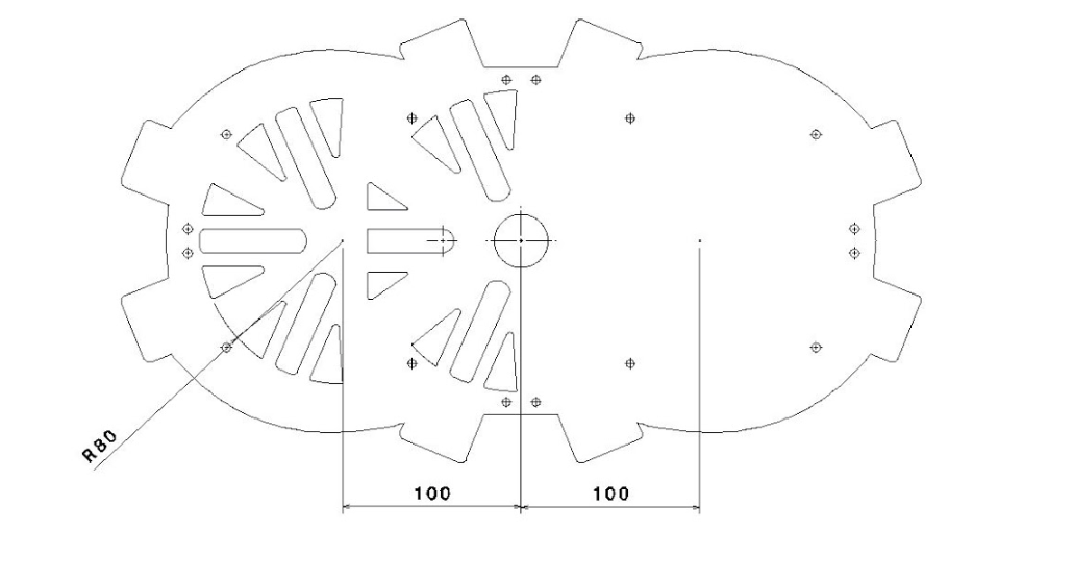
\includegraphics[keepaspectratio=true,scale=0.5]{figuras/drawing.eps}
    \caption{ Drawing Frame Central Superior}
    \label{fig:drawing}
\end{figure}

Como é possível ver na figura \label{fig:drawinfinfo}, as formas triangulares do lado esquerdo são “buracos” na qual tem como função deixar o frame mais leve, contudo, não perder sua utilidade em ser a base do VANT. O lado direito não possui esses espaços devido ser o local para alocar o desfibrilador. O lado esquerdo alocará a antena e até duas baterias , na qual serão presas por velcros, amarrados entre os “buracos” do frame. Também serão parafusadas os braços e a carcaça do VANT no mesmo.

\begin{figure}[H]
    \centering
      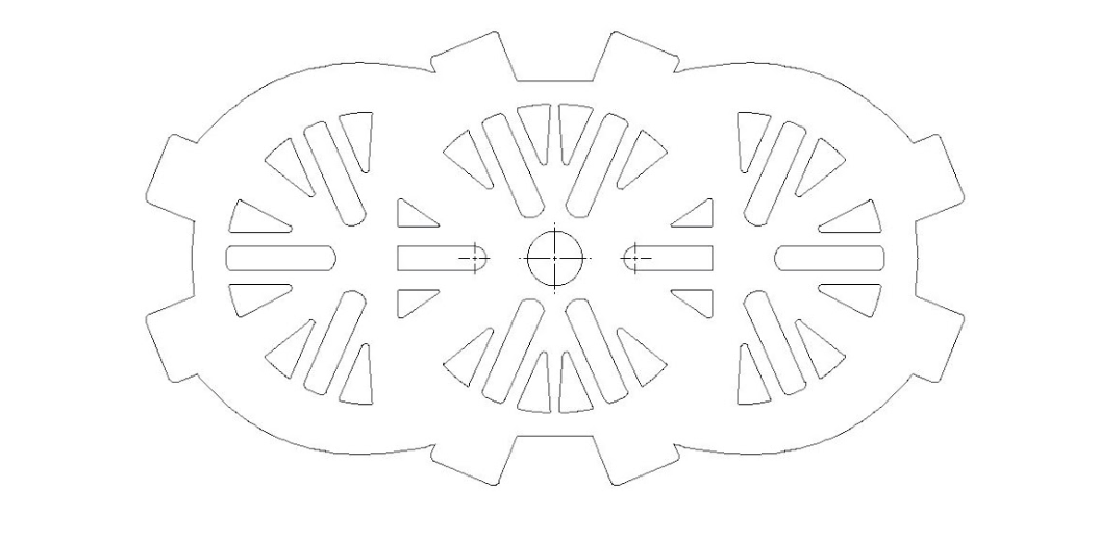
\includegraphics[keepaspectratio=true,scale=0.5]{figuras/drawinfinfo.eps}
    \caption{ Frame Central inferior.}
    \label{fig:drawinfinfo}
\end{figure}

Já o frame inferior, figura \ref{fig:drawinfinfo}, será parafusado ao trem de pouso e ao frame superior.  Ambos os frames serão unidos como mostra a figura \ref{fig:catia1}, tendo um espaço de 42mm. O espaço entre os dois frames é destinado para alocar a parte dos controladores de voo , ESC e o conjunto dos fios.

\begin{figure}[H]
    \centering
      \includegraphics[keepaspectratio=true,scale=0.5]{figuras/catia1.eps}
    \caption{Desenvolvimento do VANT no CATIA}
    \label{fig:catia1}
\end{figure}

Por meio da plataforma CATIA, foi possível idealizar o projeto EmerVANT, em escala real. Para visualizar de melhor forma, utilizou-se o KeyShot, na qual ele renderiza VANT, como mostrado na figura \ref{fig:keyshot1}:

\begin{figure}[H]
    \centering
      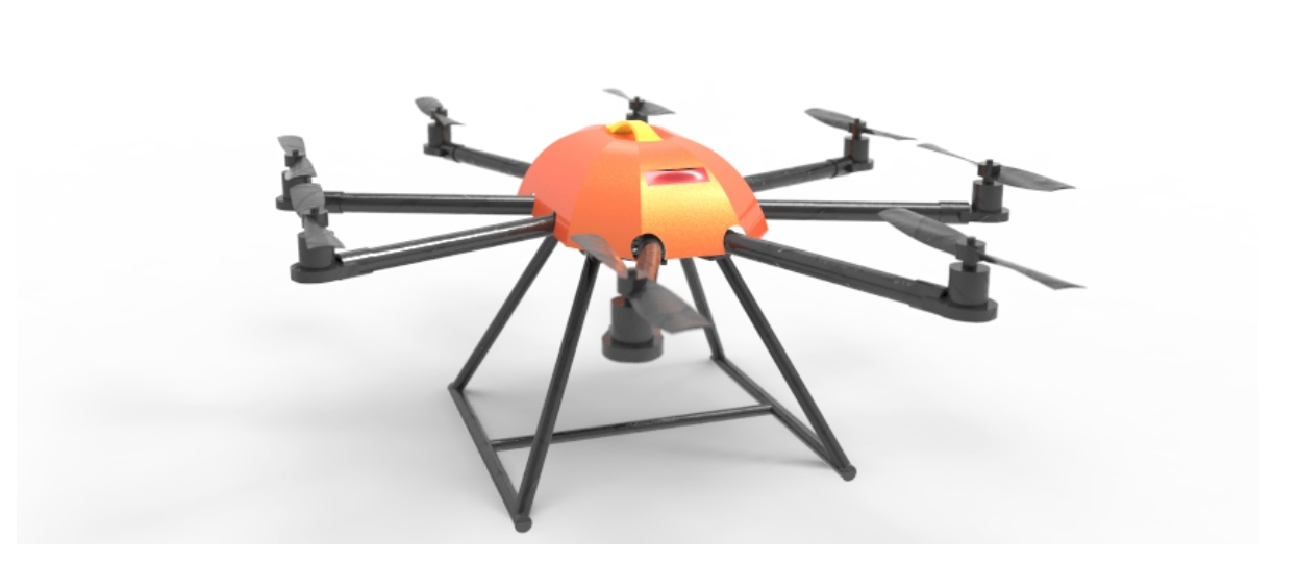
\includegraphics[keepaspectratio=true,scale=0.5]{figuras/keyshot1.eps}
    \caption{ Renderização do Projeto EmerVANT}
    \label{fig:keyshot1}
\end{figure}

O retângulo vermelho, presente na parte superior da estrutura do VANT, mostrado na figura 21, é a gaveta para retirada dos eletrodos do Desfibrilador Externo Automático, o local onde os eletrodos ficam guardados será passado para o usuário através do procedimento de instruções para a utilização do EmerVant. A central ficará responsável por dar todas as informações necessárias para a utilização do equipamento e atendimento.

\begin{figure}[H]
    \centering
      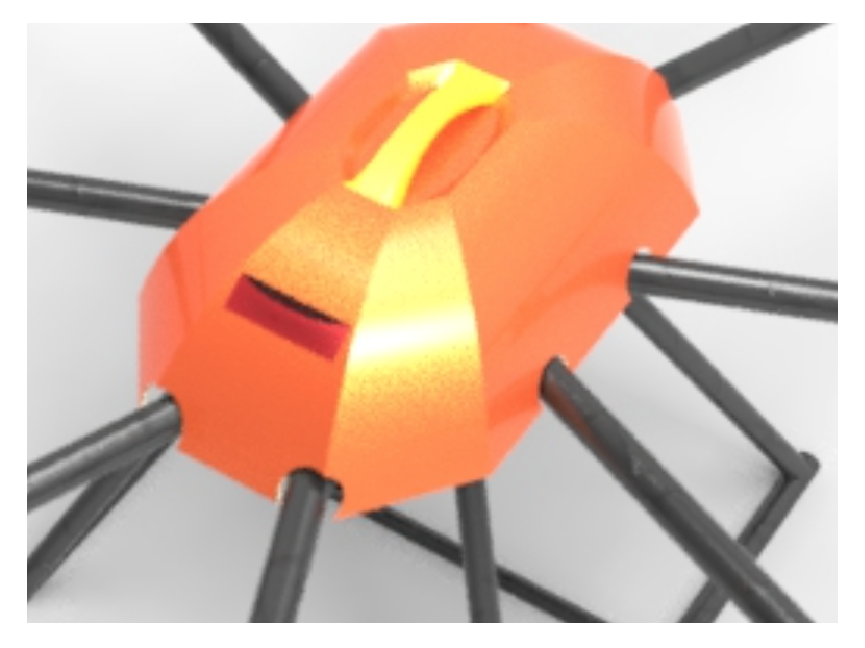
\includegraphics[keepaspectratio=true,scale=0.5]{figuras/keyshot2.eps}
    \caption{ Gaveta para eletrodos}
    \label{fig:keyshot2}
\end{figure}

\subsubsection{Análise de custos}

\indent \textbf{Frame central e trem de pouso}

Como definimos projetar alguns acessórios do VANT, como frame central, trem de pouso e a carcaça, foram levantados alguns estudos sobre como será projetado. O frame central e o trem de pouso, ambos serão projetados com fibra de carbono, pois se tratam de estruturas com características mais rígidas e resistentes para que possa suportar as tensões calculadas.

O preço do metro quadrado encontrado para esta fibra de carbono de pano liso está entre R\$150 e R\$200. Para realizar os custos de cada peça, atribuímos o valor de R\$200 o metro quadrado.

Todos os cálculos feitos a seguir são aproximações de comprimento dos componentes acima listados com uma margem de erro de 5\% para mais.

\begin{figure}[H]
    \centering
      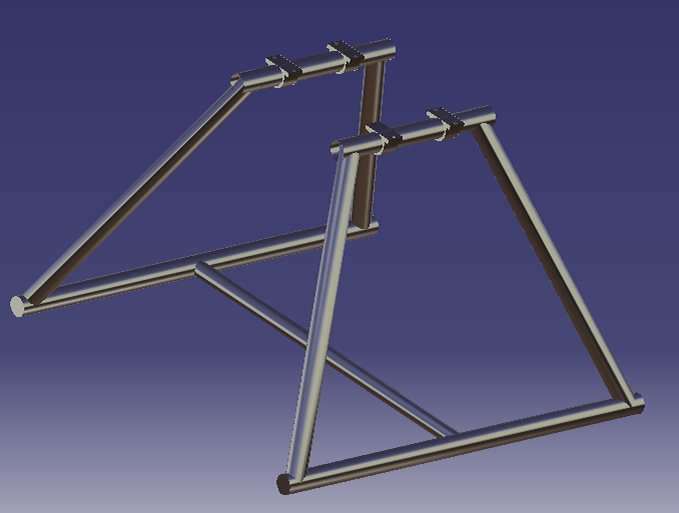
\includegraphics[keepaspectratio=true,scale=0.5]{figuras/frame_central.png}
    \caption{Trem de pouso CATIA}
    \label{fig:frame_central}
\end{figure}

Os tubos de fibra de carbono, que compõe o trem de pouso apresentado na figura \ref{fig:frame_central},
com 21 mm de diâmetro externo, 2 mm de espessura e 1m de comprimento custarão em torno de
R\$140 e R\$160 cada. O numero de tubos necessários para a construção do VANT serão de 8 devido
as varrições de comprimento de cada seção. Estas seções podem variar entre um comprimento de
251mm e 388mm.

De acordo com o preço de cada tubo, o preço total será de R\$1280. A junção destes será feita
por técnico mecânico industrial com valor de serviço de R\$20 (Guia do Estudante)\footnotemark a hora.

\footnotetext{http://guiadoestudante.abril.com.br/profissoes/engenharia-producao/automacao-industrial-684507.shtml}

Este técnico também elaborará a produção do Frame Central de acordo com os detalhes
especificados. Devido a esta peculiaridade a produção desta demorará em torno de 6 horas e as
junções das conexões das seções restantes terá tempo estimado de 16 horas, totalizando um total de
22h horas.

Portanto, o valor de número de horas a ser pagas a este técnico terá custo de no minimo
R\$440,00. Somando o preço total a ser pago para o número de tubos e horas trabalhadas, o valor total
a ser empregado nesta parte do projeto será de R\$1765,00.

\begin{table*}[!h]
\centering
    \caption{Custo de Fabricação das peças com Fibra de Carbono}
\begin{tabular}{|p{0.20\linewidth}|p{0.15\linewidth}|p{0.15\linewidth}|p{0.15\linewidth}|p{0.15\linewidth}|p{0.15\linewidth}|}
\hline

Peça & Preço& Quantidade& Horas Trabalhadas &HT x Hora técnico& Total\\ \hline
Frame Central &R\$ 22,50& 2 &3h x 2 = 6h& 6h x R\$20 = R\$120,00& R\$165,00 \\ \hline
Tubos (trem de Pouso)& R\$160,00& 8 &2h x 8 = 16h &16h x R\$20 = R\$320,00& R\$1600,00\\ \hline
\textbf{Total} & & & & & \textbf{R\$1765,00}\\ \hline

\end{tabular}
    \label{custos_carregador}
\end{table*}

\pagebreak
\indent \textbf{Carcaça}

Foi decidido que a carcaça do EmerVANT será feita através de uma impressora 3D
com o polímero ABS como material.

\indent \indent \textbf{Funcionamento da impressora 3D}

\begin{figure}[H]
    \centering
      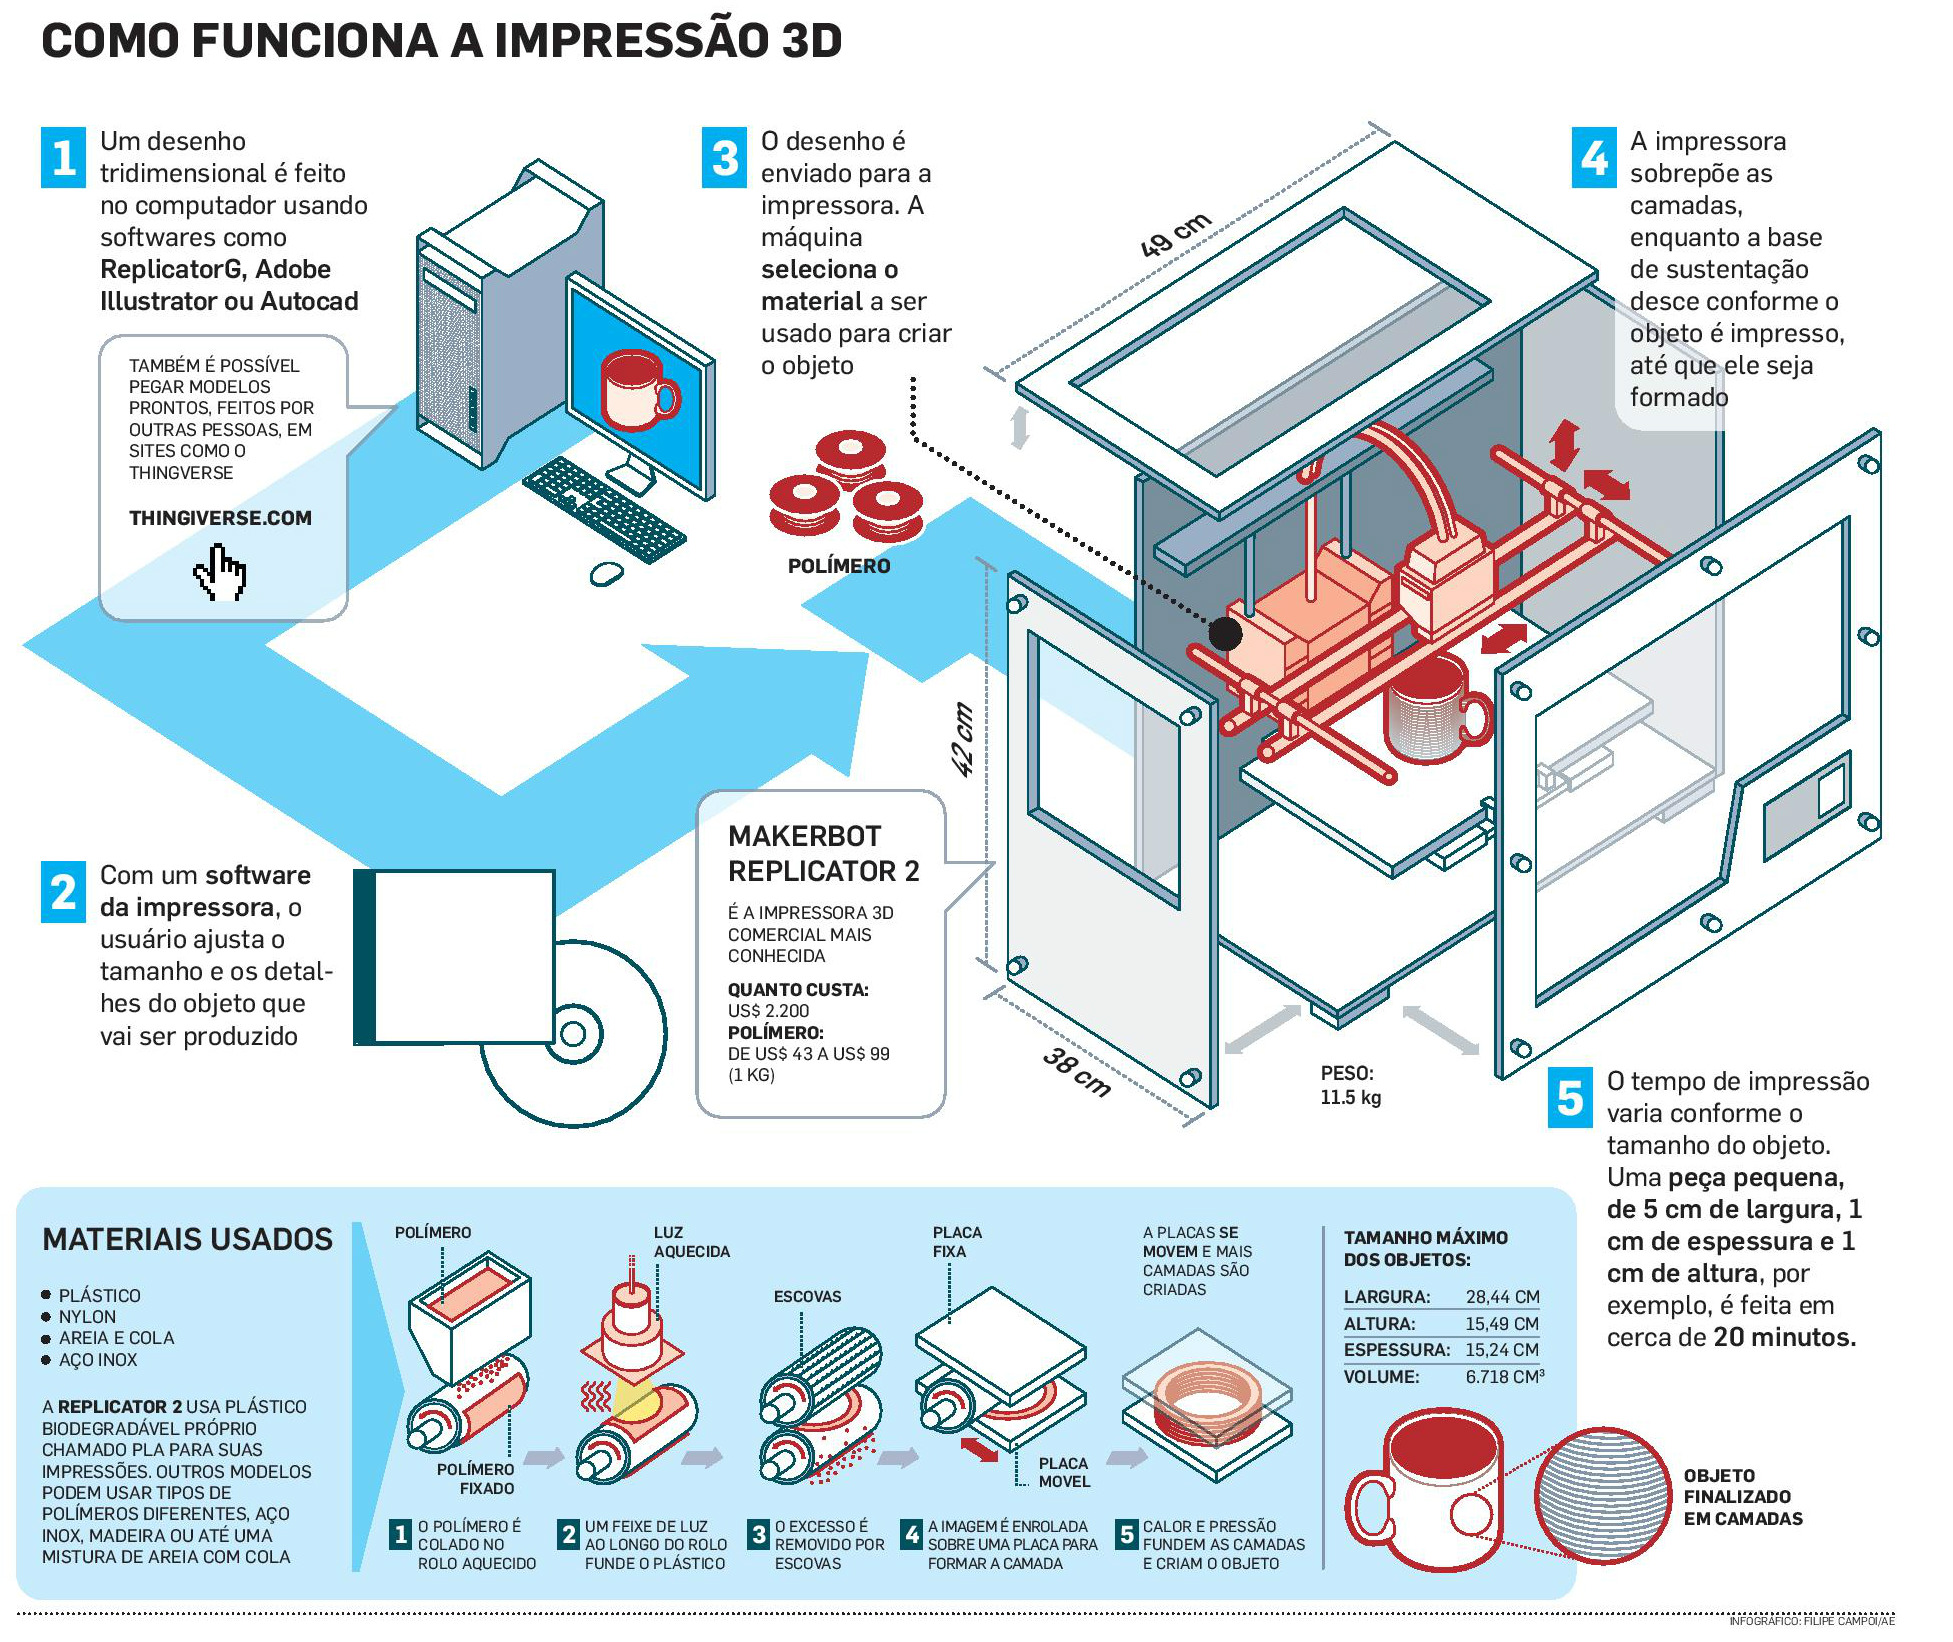
\includegraphics[keepaspectratio=true,scale=0.25]{figuras/impressao3D.jpg}
    \caption{Funcionamento de uma impressora 3D. Fonte: Fireprint}
    \label{fig:impressao3D}
\end{figure}

\footnotetext{http://www.graficafireprint.com.br/impressoras-3d/}
De acordo com o site da \textit{MakerBot}\footnotemark, as peças de filamento de plástico ABS são vendidas em quilograma, uma peça contendo um quilograma custa US\$48,00, como a carcaça do EmerVant tem aproximadamente 0,6363kg usando o polímero ABS, convém comprar somente uma  peça contendo um quilograma. Para ser enviada à Brasília as taxas de entrega resultam em US\$85,77, gerando um total de US\$133,77. Usando a cotação do dólar do dia 18/06/2015 as 17:24 de US\$3,0588, resultando assim R\$409,18.

O tempo para projetar a carcaça é de no mínimo 3 horas e o custo de um projetista atualmente no mercado é de aproximadamente R\$17,00 a hora resultando assim o custo de projeto em R\$51,00.

Foi feito um orçamento na empresa Grupo Alutech para fazer a confecção da carcaça do EmerVant usando polímero ABS na cor amarela custa no total com o frete R\$2145,00.

O custo total da carcaça do EmerVant somando projeto e material é R\$ 460,18. Se for contratada uma empresa para fazer o serviço, então o custo seria somente o de projeto e o da empresa, resultando em R\$2196,00.

\footnotetext{http://www.makerbot.com/search?q=ABS}

\indent \textbf{Braço, Hélice e Motor}

O motor, o braço e a hélice serão baseadas no VANT S1000 do fabricante DJI, o que
não será necessário projetar ambas as peças. No site \textit{Dronestore}\footnotemark é possível comprar o
conjunto motor, hélice e braço.

\footnotetext{http://www.dronestore.com.br/}

\begin{figure}[H]
    \centering
      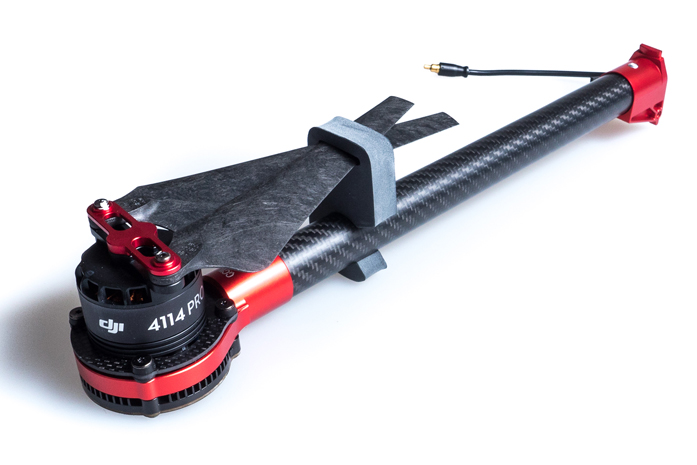
\includegraphics[keepaspectratio=true,scale=0.4]{figuras/braco_helice.jpg}
    \caption{Conjunto braço, motor e hélice. Fonte: \textit{Dronestore}}
    \label{fig:braco_helice}
\end{figure}

Conforme o verificado no site \textit{Dronestore}, o valor de um conjunto como acima, custa
R\$1654,00. Como são 8 braços, o valor total será de R\$13.232,00.

\indent \textbf{Desfibrilador e Reanimador Manual}

No caso do Desfibrilador Externo Automático (DEA), não será necessário fabricar um
para o projeto. Apenas será feito a compra de um DEA chamado \textit{HeartSine samaritan PAD
SAM 300P}. Conforme feito pesquisas para saber quanto custa, no site \textit{First Aid Product}\footnotemark, está
no preço de U\$1.600,00. Usando a cotação do dólar do dia 18/06/2015 as 17:24 de
US\$3,0588, o valor sai em R\$4.594,00.
\footnotetext{http://www.first-aid-product.com/}

No caso do Reanimador Manual, são 3 tipos de reanimador: Neonatal, Reanimador Infantil e Reanimador Adulto a partir dos 13 anos. R\$140,00 - cada unidade\footnotemark. 
Será realizado a compra do conjunto de Reanimadores da marca PROTEC\footnotemark.

\footnotetext{http://www.medicalfast.com.br/}
\begin{figure}[H]
    \centering
      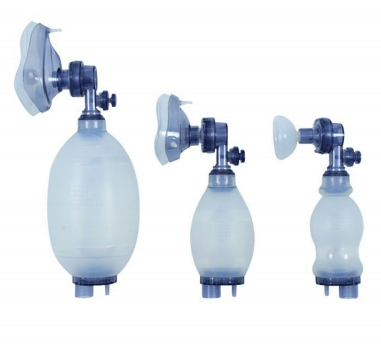
\includegraphics[keepaspectratio=true,scale=0.4]{figuras/reanimadores.png}
    \caption{Tipos de Reanimadores Manuais. Fonte: PROTEC}
\end{figure}

\footnotetext{http://www.protec.com.br/}
No Total, o conjunto de reanimadores custará R\$420,00.

\indent \textbf{Total}

\begin{table*}[!h]
\centering
    \caption{Custos totais da parte estrutural}
\begin{tabular}{|p{0.20\linewidth}|p{0.20\linewidth}|p{0.20\linewidth}|}
\hline

Peça &Quantidade& Preço\\ \hline
Tubos (Trem de pouso)&8 &R\$1600,00\\ \hline
Frame Central &2 &R\$165,00\\ \hline
Braço, hélice e motor &8 &R\$13.232,00\\ \hline
Desfibrilador &1 &R\$4.594,00\\ \hline
Reanimador &3 &R\$420,00\\ \hline
Total& &R\$20.011,00\\ \hline
\end{tabular}
\end{table*}

O conjunto estrutural do EmerVANT terá um valor minimo de R\$20.011,00, desconsiderando a parte controladora do VANT.